\chapter{Results}
\label{chap:Results}

\section{Maximum edge weight experiment results}
\label{sec:results_maximum_edge_weight}

Experiment described in section \ref{sec:experiment_maximum_edge_weight} was
performed on both implementations and construction time and execution time of
operations were measured. Execution time per one operation is showed in the
following chart.

\begin{figure}[H]
\centering
\hsize=1.1\hsize
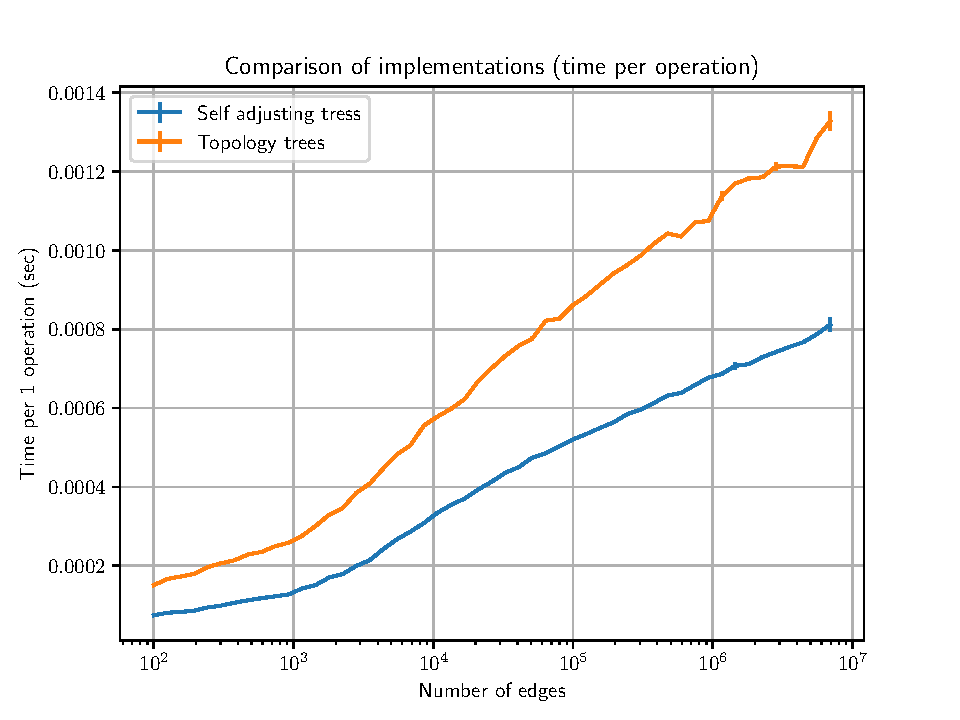
\includegraphics[width=\hsize]{charts/maximum_edge_weight_op.pdf}
\caption{Chart showing time per operation in the maximum edge weight experiment}
\end{figure}

Results show that both implementations have the same asymptotic time complexity
but as have been expected implementation with topology trees have larger
multiplicative constant.

Despite expectations this multiplicative constant is relatively small --
according to measured data the implementation with topology trees for larger
inputs (more than $10^4$ edges) is only $1.58$ to $1.68$ times slower than the
implementation which uses self adjusting trees.

\vfill\eject %% PRINTHACK

\subsubsection{Time of construction}

Initial construction time measured per one edge of the initial underlying tree
is showed in the following figure. It shows some anomaly for small number of
edges (see bigger standard deviation in the beginning) but from tree size of
$10^4$ edges it stabilizes.

It shows that the implementation based on self adjusting trees could initialize
in approximately half time than the implementation based on topology trees,
which corresponds to time per operation in the previous chart.

\begin{figure}[H]
\centering
\hsize=1.1\hsize
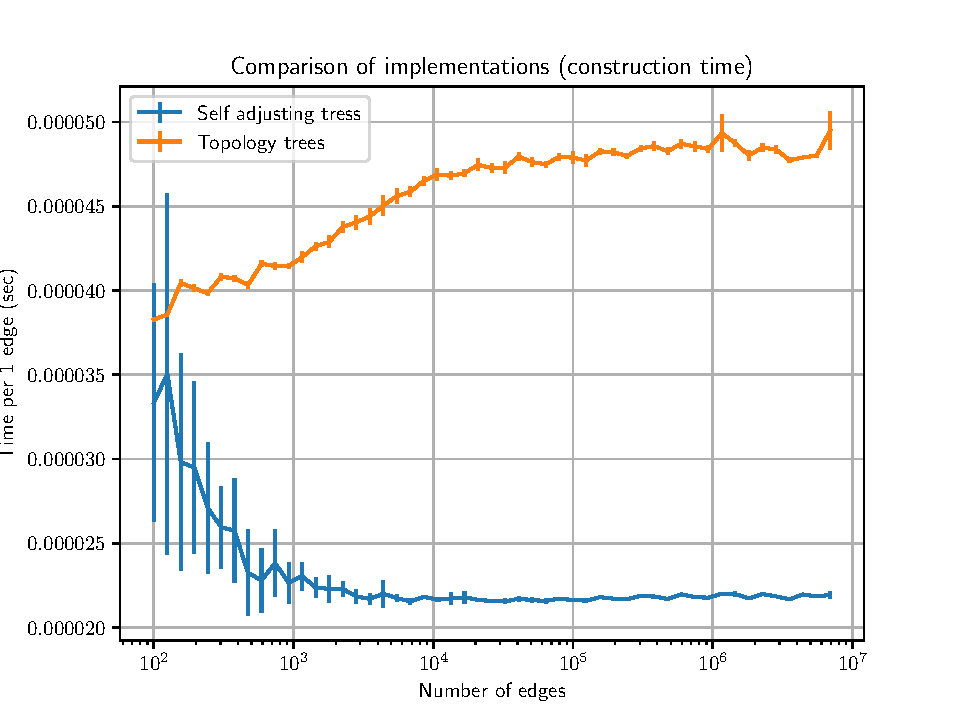
\includegraphics[width=\hsize]{charts/maximum_edge_weight_construction.pdf}
\caption{Chart showing construction time per one edge in the maximum edge weight
experiment}
\end{figure}

\vfill\eject %% PRINTHACK

\section{Edge 2-connectivity experiment results}
\label{sec:results_edge_2_connectivity}

Similarly to the previous experiment the experiment described in the section
\ref{sec:experiment_edge_2_connectivity} was performed on both implementations
(on second with normal updates and with expensive updates turned off during
query). Construction time (time to insert all initial edges) and execution time
of all operations and execution time on only query operations were measured.

\todo{Results from edge 2-connectivity experiment}
